\documentclass[../main]{subfiles}
\begin{document}

\chapter{Support Vector Machine}
\begin{introduction}
\item Conditioned optimization
\item Unstrict-Condition optimization
\item KKT condition
\item Support Vector Machine
\end{introduction}
Support Vector Machine (SVM) is also a binary classification model, often introduced as an alternative to logistic regression, since—as we have discussed in the previous chapter—logistic regression has several notable limitations. SVM provides an elegant framework that allows us to transfer powerful results and intuition from optimization theory into machine learning.
\section{Conditioned Optimization}
Unlike the unconstrained optimization problems we studied earlier, the support vector machine is originally formulated as a \textbf{constrained optimization problem}. This distinction is fundamental. In mathematics, unconstrained optimization is defined as:
\begin{equation}
    \argmin_x f(x)
\end{equation}
When we deal with constrained optimization, we add an auxiliary constraint $h(x)=0$ (where both $f(x)$ and $g(x)$ are differentiable). Considering the geometric meaning of the gradient, we observe:

\begin{enumerate}
    \item For any point on the surface defined by $g(x)$, the gradient $\nabla g(x)$ must be orthogonal to the surface.
    \item For any critical point $x^*$ that achieves a local minimum, the gradient $\nabla f(x^*)$ must also be orthogonal to the surface.
\end{enumerate}

\begin{note}
    The second property can be understood by analogy with electrostatics: near a conductor, the electric field must be orthogonal to the surface. Otherwise, there would be a component of the field (gradient) along the constrained sub-hypersurface, violating equilibrium.
\end{note}
Combining the two conditions above, we obtain the \textbf{necessary} condition for a local minimum point:
\begin{equation}
    \exists \,\lambda \quad \text{s.t.} \quad \nabla f(x^*) + \lambda \nabla h(x^*) = 0 .
\end{equation}

\begin{figure}[H]
    \centering
    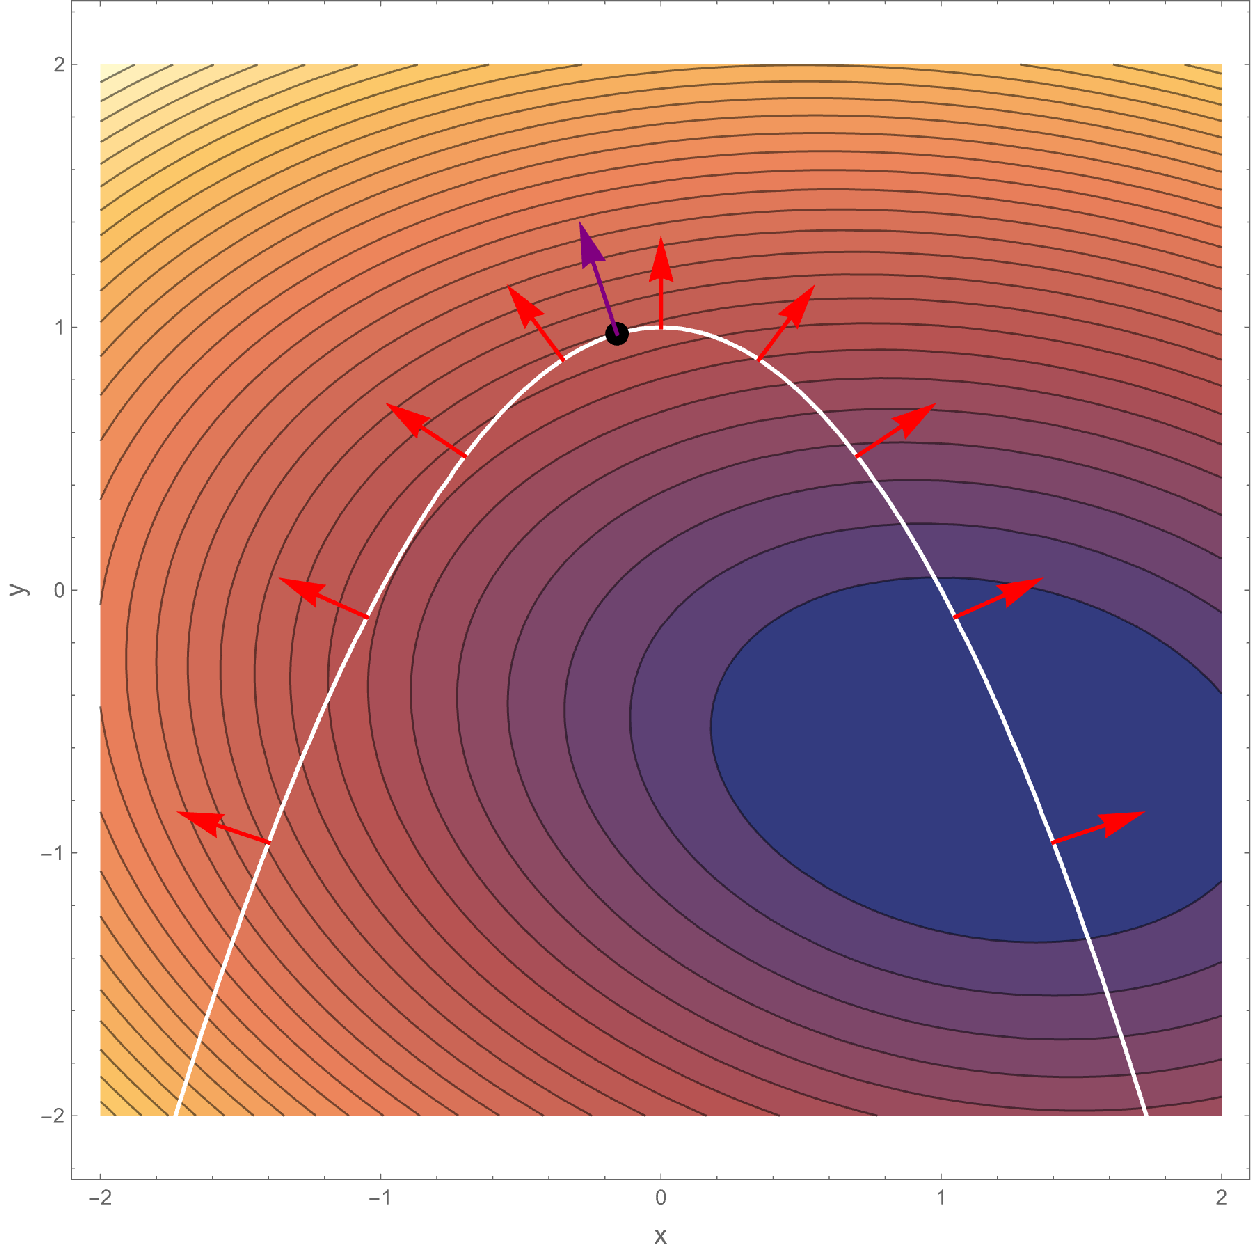
\includegraphics[width=0.5\textwidth]{../../fig/fig1.pdf}
    \caption{Illustration of the necessary condition for constrained local minima.}
    \label{2-lr}
\end{figure}

\begin{remark}
    In some contour examples, the constraint condition does not cover the entire space.  
    In such cases, the above equation may \emph{not} always be satisfied.
\end{remark}

Now we introduce the \emph{Lagrangian function}, which plays a central role in optimization theory:
\begin{equation}
    L(x, \lambda) := f(x) + \underbrace{\lambda}_{\text{Lagrange Multiplier}} h(x).
\end{equation}
Extending to the case of multiple constraints, the Lagrangian is defined as:
\begin{equation}
    L(x,\lambda) := f(x) + \sum_{i=1}^k \lambda_i h_i(x).
\end{equation}

\begin{theorem}
    If $x^*$ is a local minimum point, then there exists a set of multipliers $\lambda = (\lambda_1,\dots,\lambda_k)$ such that
    \begin{equation}
        \begin{cases}
            \nabla_x L(x^*, \lambda) = 0, \\
            \nabla_\lambda L(x^*, \lambda) = 0.
        \end{cases}
    \end{equation}
    The first condition corresponds to the stationarity (minimum) condition, while the second condition enforces the constraints.
\end{theorem}

\begin{corollary}
    In multi-constrained problems, the minimum condition becomes
    \begin{equation}
        \nabla f(x^*) + \sum_{i=1}^k \lambda_i \nabla h_i(x^*) = 0.
    \end{equation}
\end{corollary}
\begin{remark}
    In higher dimensions, the constrained submanifold may possess certain free variables that can be chosen arbitrarily while still satisfying the minimum condition. 
    Specifically, if $\nabla f(x^*)$ cannot be expressed as a linear combination of $\nabla h_1(x^*)$ and $\nabla h_2(x^*)$, it is possible to continue optimizing along the intersection submanifold defined by $h_1=0$ and $h_2=0$.  
    Therefore, it must be emphasized that the above equation provides only a \textbf{necessary condition}, not a sufficient one.
\end{remark}

\begin{figure}[H]
    \centering
    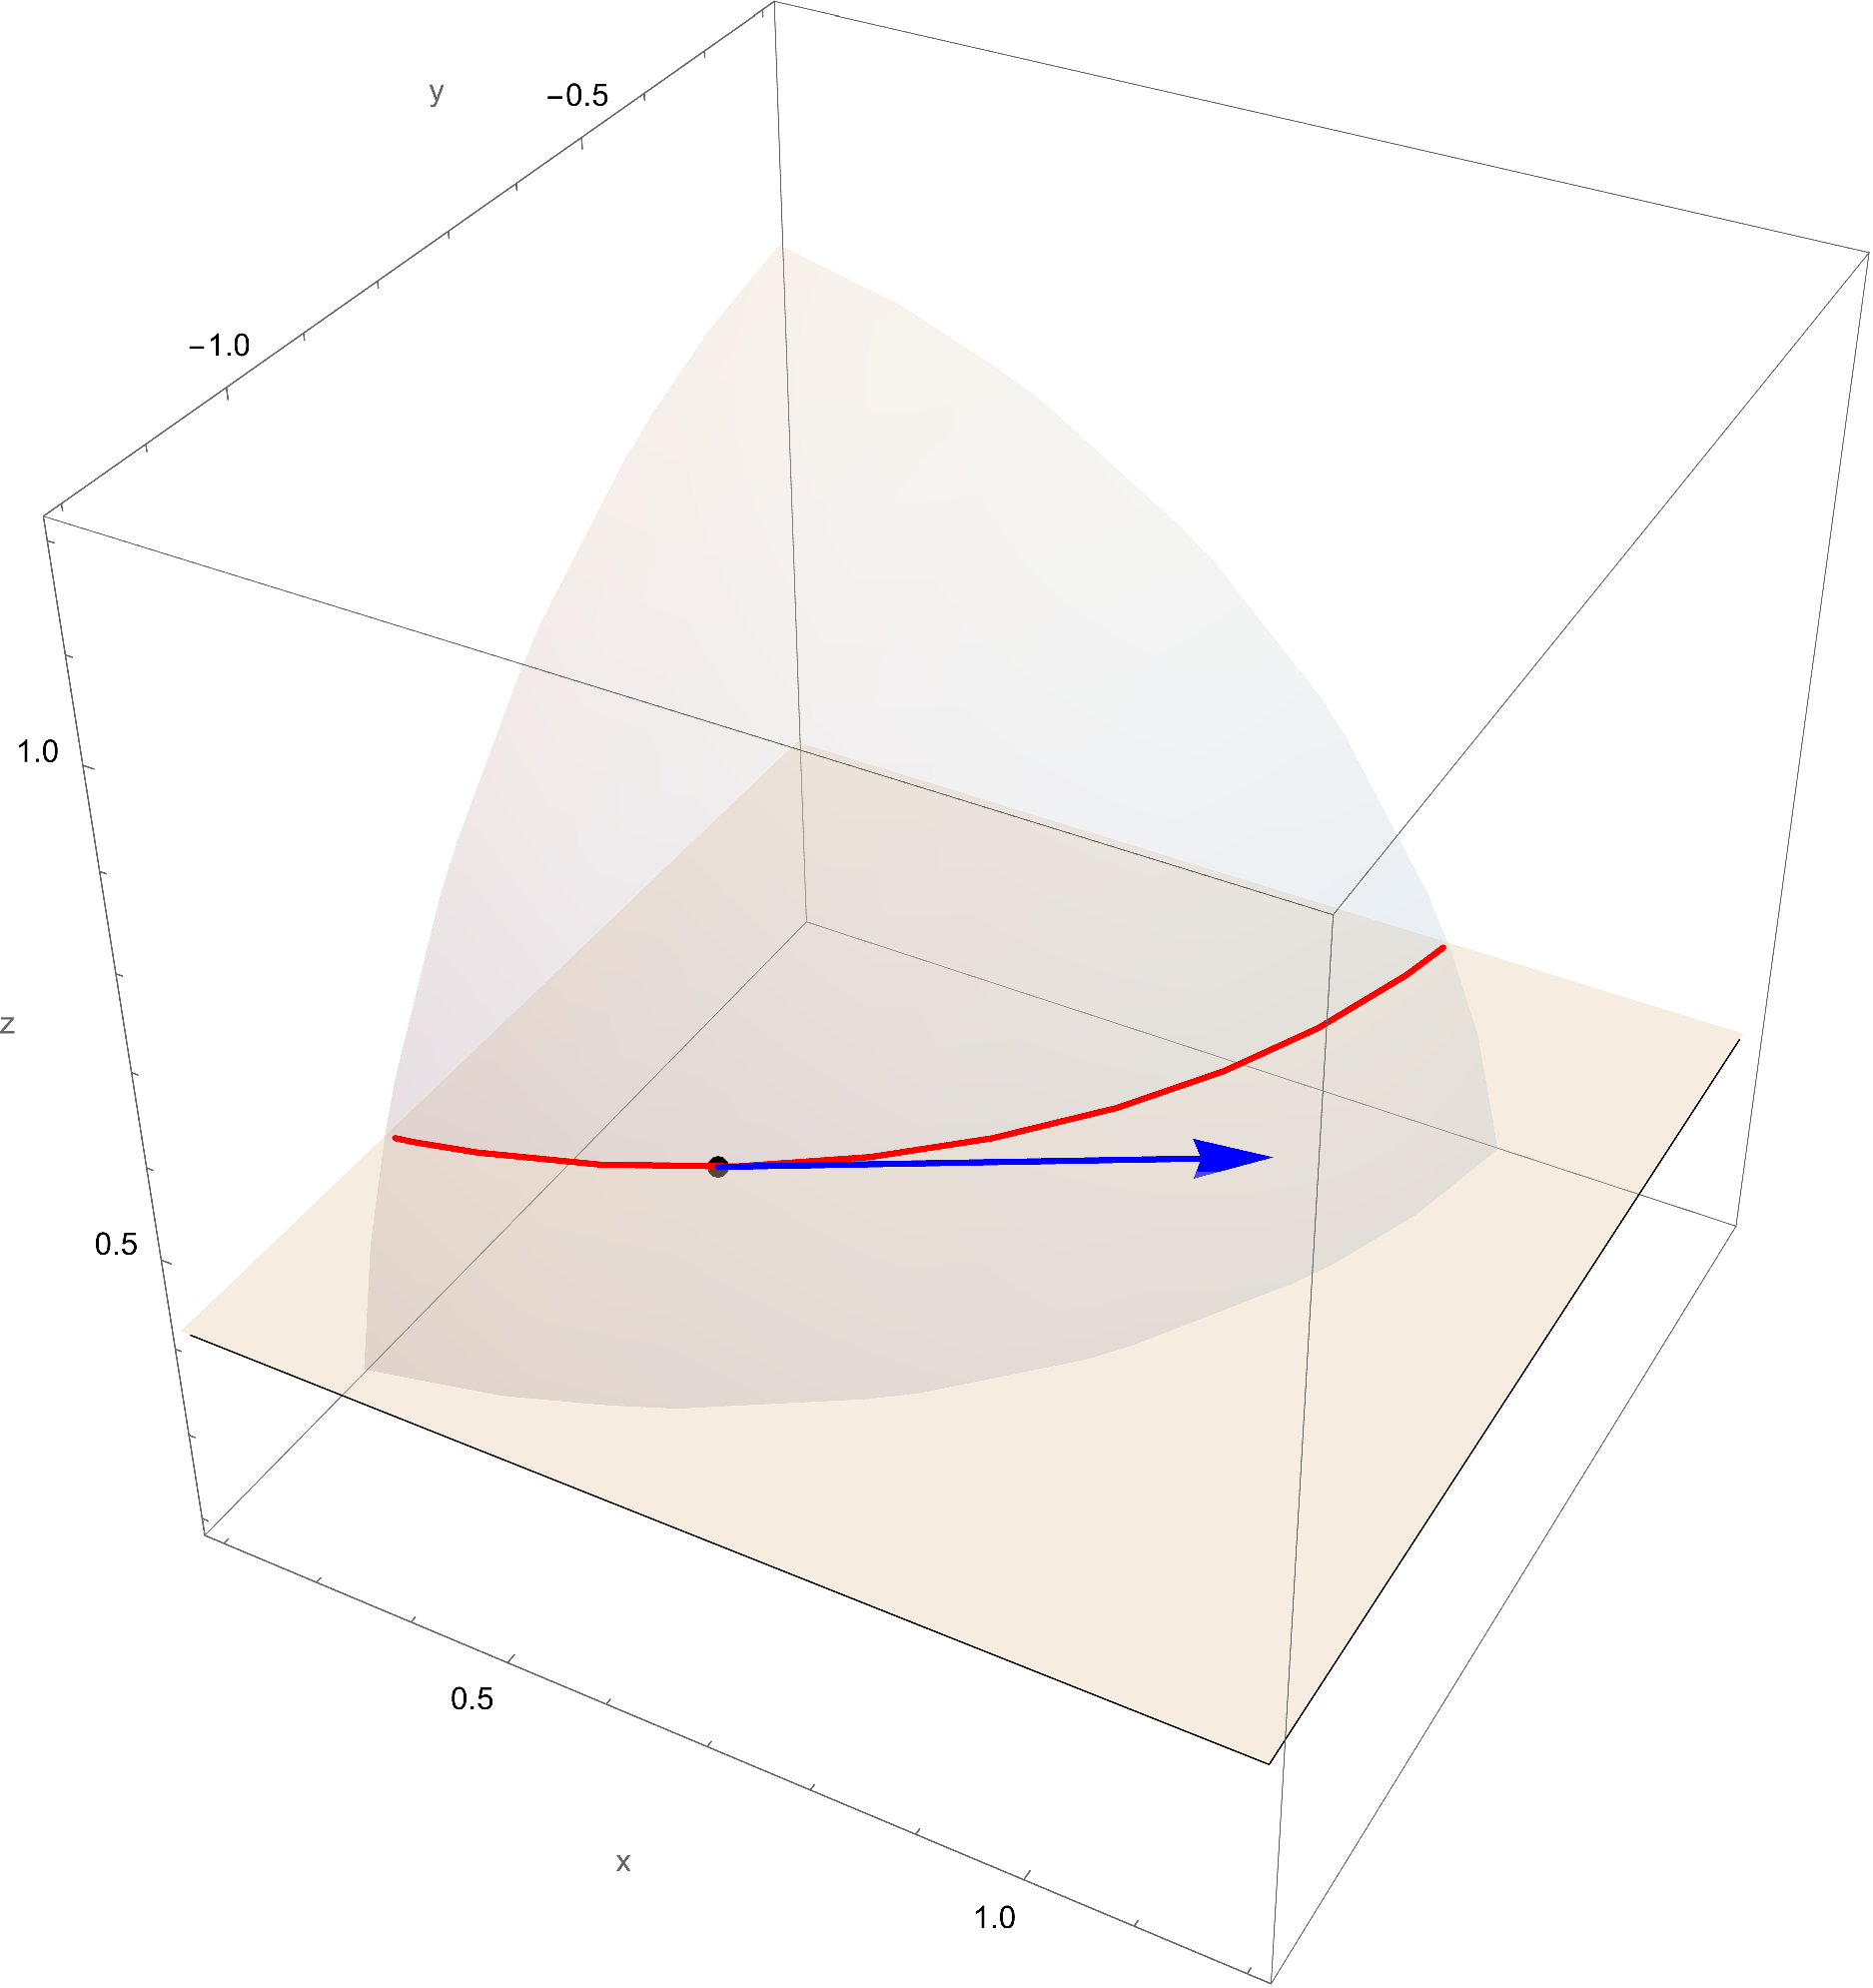
\includegraphics[width=0.5\textwidth]{../../fig/fig2.pdf}
    \caption{Illustration of optimization along the intersection of two constraint manifolds.}
    \label{2-lr}
\end{figure}

\begin{example}
    Consider the following constrained optimization problem:
    \begin{equation}
        \argmin_{x_1, x_2} \; x_1 + x_2
    \end{equation}
    subject to the constraint
    \begin{equation}
        (x_1 - 1)^2 + x_2^2 - 1 = 0.
    \end{equation}
\end{example}
\begin{solution}
    $1-\sqrt{2}$.
\end{solution}

\begin{note}
    The Lagrange multiplier method can provide critical points, but these do not always correspond to the minimum solution.
\end{note}

\begin{note}
    In convex settings, any local minimum is also a global minimum.
\end{note}

A new problem arises: what if we have an inequality constraint instead of a strict equality, i.e., $g(x) \leq 0$?

\begin{remark}
\section{Unstrict-Condition optimization}
    We assume the feasible set of $x$ is compact; otherwise, the existence of a minimum may be problematic.
\end{remark}

By gradient analysis, we obtain:
\begin{enumerate}
    \item For any point on the surface $g(x)=0$, $\nabla g(x)$ is orthogonal to the surface and points outward from the feasible region $g(x)\leq 0$.  
    This is straightforward, since $\nabla g(x)$ indicates the steepest direction of increase.
    \item For a local minimum point $x^*$:
    \begin{enumerate}
        \item If $x^*$ lies on the surface $g(x)=0$ (in other words, the constraint is \emph{active}), then $-\nabla f(x^*)$ must be aligned with $\nabla g(x^*)$.  
        Equivalently, $\exists \,\mu > 0$ such that 
        \[
            \nabla f(x^*) + \mu \nabla g(x^*) = 0.
        \]
        \item If $x^*$ does not lie on the surface, i.e., $g(x)<0$ (the constraint is \emph{inactive}), we simply require $\nabla f(x^*)=0$.  
        In the unified form above, this corresponds to $\exists \,\mu=0$ such that 
        \[
            \nabla f(x^*) + \mu \nabla g(x^*) = 0.
        \]
    \end{enumerate}
\end{enumerate}

\begin{note}
    How should we understand the meaning of an ``active'' constraint?  
    When the inequality constraint is not tight (i.e., $g(x)<0$), it does not affect gradient descent optimization.  
    In this case, the constraint is effectively absent, which is why we call it \emph{inactive}.
\end{note}
Again, we define the Lagrangian as
\begin{equation}
    L(x, \mu) = f(x) + \mu g(x),
\end{equation}
where $g(x)$ denotes the inequality constraint function.  
Following the same steps as in the equality-constrained case, we obtain:

\begin{theorem}
    If $x^*$ is a local minimum point, then
    \begin{equation}
        \begin{cases}
            \nabla L(x^*, \mu) = 0, \\
            g(x^*) \leq 0, \\
            \mu \geq 0, \\
            \mu \cdot g(x^*) = 0.
        \end{cases}
    \end{equation}
\end{theorem}

The last condition (the \emph{complementary slackness}) unifies the boundary and interior cases, since either $g(x^*)=0$ (active constraint) or $\mu=0$ (inactive constraint) must hold.
\section{General Case}
In the most general case, we consider the optimization problem
\begin{equation}
    \argmin_x f(x)
\end{equation}
subject to equality constraints $h_i(x) = 0, \; i \in [k]$, and inequality constraints $g_j(x) \leq 0, \; j \in [l]$.  

The corresponding Lagrangian is defined as
\begin{equation}
    L(x, \lambda, \mu) := f(x) + \sum_{i \in [k]} \lambda_i h_i(x) + \sum_{j \in [l]} \mu_j g_j(x).
\end{equation}

In this setting, a local minimum $x^*$ must satisfy a series of conditions known as the \textbf{Karush--Kuhn--Tucker (KKT) conditions}:

\begin{theorem}[KKT Conditions]
    If $x^*$ is a local minimum point, then there exist multipliers $(\lambda, \mu)$ such that
    \begin{equation}
        \begin{cases}
            \nabla L(x^*, \lambda, \mu) = 0, & \\
            h_i(x^*) = 0, & \forall i \in [k],  \\
            g_j(x^*) \leq 0, & \forall j \in [l], \\\
            \mu_j \geq 0, & \forall j \in [l], \\
            \mu_j \cdot g_j(x^*) = 0, & \forall j \in [l]. 
        \end{cases}
    \end{equation}
\end{theorem}

In most cases, the above conditions cannot be solved explicitly in closed form.  

\section{Support Vector Machine}
\subsection{Hard Margin}
Consider a linearly separable dataset $\{(x_i, y_i)\}$ with $y_i \in \{0,1\}$, and a linear model
\begin{equation}
    f(x) = w^\top x + b.
\end{equation}
Although introducing a regularization term can make the solution unique by adjusting the hyperparameter $\lambda$, this does not resolve the issue of determining which solution $f(x;\lambda)$ is preferable among all possible choices, since $\lambda$ is itself arbitrary.

Our goal is for the model to generalize well to test data drawn from the same distribution as the training set.  
A direct and intuitive way to achieve this is to choose the separating hyperplane that maximizes the distance between the plane and the nearest datapoints.

\begin{definition}[Support Vectors]
    The datapoints that lie closest to the separating hyperplane, such that the vectors orthogonal to the hyperplane connect the hyperplane to these datapoints, are called \emph{support vectors}.
\end{definition}
%%%
In the case of SVM, we aim to find the \textbf{Max-Margin Classifier}, i.e., the hyperplane that maximizes the minimum margin across all training points.  
Here, the \emph{margin} refers to the distance from a point to the hyperplane, which is equivalently the norm of the vector associated with its support vector.

\begin{remark}
    Why does $w^\top x + b = 0$ represent a hyperplane?  
    Consider the hyperplane through the origin, given by $w^\top x = 0$.  
    Translating this plane until it passes through some point $x_0 \notin \{x \mid w^\top x = 0\}$, we obtain
    \[
        w^\top (x - x_0) = 0.
    \]
    Setting $-w^\top x_0 = b$, we recover the general hyperplane equation
    \[
        w^\top x + b = 0.
    \]
\end{remark}

\begin{remark}
    Note that the interpretation of $b$ differs between the two cases $y = w^\top x + b$ and $0 = w^\top x + b$.  
    In the latter, we can observe that $|b| = \|w\| \|x_0\|$, which corresponds to the offset determined by $x_0$.
\end{remark}
The distance between a datapoint and the hyperplane is given by:
\begin{theorem}
    \begin{equation}
        d = \frac{|w^\top x + b|}{\|w\|}. \label{3.15}
    \end{equation}
\end{theorem}

Geometrically, we obtain:

\begin{figure}[H]
    \centering
    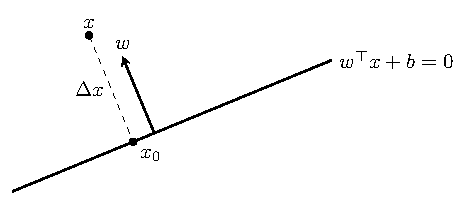
\includegraphics{../../tikz/3/1.pdf}
    \caption{Support Vector Machine.}
    \label{2-lr}
\end{figure}

\begin{enumerate}
    \item Consider
    \[
        \begin{cases}
            x_0 + \Delta x \dfrac{w}{\|w\|} = x, \\
            w^\top x_0 + b = 0,
        \end{cases}
    \]
    so that
    \begin{align*}
        w^\top x_0 + w^\top \Delta x \frac{w}{\|w\|} &= w^\top x, \\
        -b + w^\top \Delta x \frac{w}{\|w\|} &= w^\top x, \\
        \Delta x \|w\| &= w^\top x + b.
    \end{align*}
    This matches exactly the expression we obtained in \eqref{3.15}.
    
    \item From the Lagrangian perspective:
    \begin{align*}
        \argmin_{x_0}\; \frac{1}{2}\|x - x_0\|^2 
        &\quad\Rightarrow\quad 
        L(x_0,\lambda) = \frac{1}{2}\|x - x_0\|^2 + \lambda (w^\top x_0 + b), \\
        \text{s.t. } w^\top x_0 + b &= 0, \\
        \nabla_{x_0} L(x_0, \lambda) = 0 
        &\quad\Rightarrow\quad x_0 - x + \lambda w = 0, \\
        \nabla_\lambda L(x_0, \lambda) = 0 
        &\quad\Rightarrow\quad w^\top x_0 + b = 0.
    \end{align*}
    This leads to the same solution as above.
\end{enumerate}
When $\Delta > 0$, the point $x$ lies on the positive side of the hyperplane;  
when $\Delta = 0$, $x$ lies exactly on the hyperplane;  
and when $\Delta < 0$, $x$ lies on the negative side.  

We define
\begin{equation}
    \gamma_i = \frac{y_i(w^\top x_i + b)}{\|w\|}
\end{equation}
to incorporate both the label information and the margin (distance to the hyperplane).  
If $\gamma_i > 0$, the point $x_i$ is correctly classified.  

Define the margin
\begin{equation}
    \gamma = \min_{i \in [n]} \gamma_i,
\end{equation}
and the SVM optimization problem can be formalized as
\begin{equation}
    \argmax_{w,b} \; {\color{red}{\gamma}}, 
    \quad \text{s.t. } \forall i, \; \frac{y_i (w^\top x_i + b)}{\|w\|} \geq \gamma.
\end{equation}

This formulation seems problematic, since $\gamma$ is not independent of $(w,b)$.  
To resolve this, suppose $(x_0, y_0)$ is a point achieving the minimum margin $\gamma_i$.  
Then
\begin{equation}
    \gamma = \frac{y_0 (w^\top x_0 + b)}{\|w\|}.
\end{equation}
Thus, the SVM objective can be reformulated as
\begin{equation}
    \argmax_{w,b} \; \frac{y_0 (w^\top x_0 + b)}{\|w\|}, 
    \quad \text{s.t. } \forall i, \; y_i (w^\top x_i + b) \geq y_0 (w^\top x_0 + b).
\end{equation}
We claim that we can make $y_0(w^\top x_0 + b)$ arbitrarily large without affecting the result.

\begin{remark}
    This is immediate: scaling $w$ and $b$ by the same factor $\lambda$ does not change the optimization, since the numerator $y_i(w^\top x_i + b)$ and the denominator $\|w\|$ both scale by $\lambda$, and the factor cancels during simplification.
\end{remark}

Thus, we may set $y_0(w^\top x_0 + b) = 1$.  
Define the \emph{functional margin} as $y_i(w^\top x_i + b)$ and the \emph{geometric margin} as $y_i(w^\top x_i + b)/\|w\|$.  
Since the functional margin alone has no intrinsic meaning, it is natural to rescale it by setting the norm of the support vector to unity.  

This yields the primal form of the SVM optimization problem:
\begin{equation}
    \argmax_{w,b} \frac{1}{\|w\|}, 
    \quad \text{s.t. } y_i (w^\top x_i + b) \geq 1 \quad \forall i,
\end{equation}
which is equivalent to
\begin{equation}
    \argmin_{w,b} \frac{1}{2} \|w\|^2, 
    \quad \text{s.t. } y_i (w^\top x_i + b) \geq 1 \quad \forall i.
\end{equation}

In other words, the goal is to separate the dataset correctly while ensuring a sufficient margin, and simultaneously minimizing the norm of $w$.  
This principle is known as \textbf{Structural Risk Minimization} (SRM).

\begin{remark}
    Unlike logistic regression, datapoint far from separate hyperplane won't contribute loss. That is, only small subset of dataset is active as a constraint.
\end{remark}
\begin{proposition}
    SVM is a convex quadratic programming, and we can solve it in poltnomial time with standard package.
\end{proposition}
\begin{problem}
\begin{enumerate}
    \item What if the dataset is not linearly separable?
    \item Wht if $\gamma$ too small because of outliers?
\end{enumerate}
\end{problem}
\end{document}